\chapter{Stato dell'arte}
\begin{comment}
Cosa devo mettere in questa sezione??

- L'obbiettivo è arrivare a parlare del modello LAMA, quindi effetturò una serie di passaggi per passare dai primi modelli gan generativi
(goodfellow2014generative), che erano i più utilizzati per generare immagini di alta qualità fino a poco tempo fa.
Per poi passare per pix2pix per introdurre le reti generative condizionate, e quindi dopo una breve introduzione al problema dell'inpainting arrivare a parlare di LAMA.

SCALETTA:
    - first gan (goodfellow2014generative)
    - DCGAN
    - WGAN
    - pix2pix
    - LAMA
\end{comment}

In questa sezione verranno mostrati i principali modelli generativi basati su architettura GAN, che sono stati utilizzati negli ultimi anni, partendo dal primo modello proposto da Goodfellow et al. \cite{goodfellow2014generative} capostipite di questa famiglia di modelli passando per alcune delle principali innovazioni proposte da altri autori, fino ad arrivare al modello LAMA \cite{suvorov2021resolutionrobust}, il quale è stato preso come base per questo progetto e riadattato per l'\textit{inpainting} condizionato. 

\section{Il primo modello GAN}
Nel 2014 Ian Goodfellow et al. \cite{goodfellow2014generative} hanno proposto il primo modello generativo basato su architettura GAN (\textit{Generative Adversarial Neural Network}).
Questa pubblicazione ha segnato un punto di svolta nella ricerca dei modelli di deep learning generativi, i quali fino ad allora erano
basati su architetture come gli \textit{autoencoder} o le \textit{deep Boltzmann machines} (DBM) che non sono in grado di generare dati di alta qualità,
o se arrivano a buoni risultati tipicamente hanno una distribuzione molto concentrata intorno ai dati del training set, dunque raggiungendo una scarsa generalizzazione.

\begin{comment}
    Next paragraphs:
    - che cos'è un modello generativo basato su architettura gan
        - struttura basilare (discriminator, generator).
    - come funziona il training e la loss function originaria (bce) con riferimenti al gradiente e alla necessità di un addestramento alternato
\end{comment}

\subsection{L'adversarial training}
Il modello GAN proposto in questa ricerca si componeva di due attori principali, il \textit{discriminatore} $\mathbf{D}$ e il \textit{generatore} $\mathbf{G}$
, due modelli neurali MLP, che si affrontano in un gioco a due giocatori a somma zero.
Il generatore in questo gioco ha il compito di generare dati che siano in grado di ingannare il discriminatore, che ha il compito opposto di distinguere i dati che 
provengono dal generatore da quelli che provengono dal training set. Il gioco viene detto a somma zero in quanto il successo di uno dei due attori è sempre
associato al fallimento dell'altro, dunque il gioco non può mai vedere entrambi i giocatori vincitori. 
I due diventeranno gradualmente sempre più bravi nel loro compito fino al punto
in cui la distribuzione dei dati generati dal generatore sarà molto simile a quella dei dati del training set.
Una componente importante che differenzia le GAN da altri modelli generativi è la presenza di un input random $\mathbf{z}$, che viene passato al generatore
, questo fatto porta il generatore ad una maggiore generalizzazione in quanto questo cercherà naturalmente una 
funzione che leghi il suo output ad un input \textit{random}, dunque la sua distribuzione sarà più ampia e non strettamente concentrata intorno ai dati del training set
come nel case dei \textit{variational autoencoder} (VAE).

A questo punto, iniziamo ad elencare le componenti che utilizzeremo per descrivere matematicamente come funziona la procedura di addestramento 
di questa GAN.

\begin{itemize}
    \item $\mathbf{x}$: esempio proveniente dal training set, $\mathbf{x \in \mathbb{R}^n}$.
    \item $\mathbf{z}$: input casuale, utilizzato per determinare una mappatura nello spazio dei dati, $\mathbf{z \in \mathbb{R}^m}$.
    \item $\mathbf{y}$: uscita del discriminatore, $\mathbf{y \in [0,1]}$, esprime la probabilità che x sia reale.
    \item $\mathbf{\hat{y}}$: uscita desiderata, $\mathbf{\hat{y} \in \{0,1\}}$, può assumere solo due valori, vero o falso.
    \item $\mathbf{p_z}$: distribuzione dei vettori casuali passati al generatore.
    \item $\mathbf{p_g}$: distribuzione dei dati generati dal generatore.
    \item $\mathbf{p_{_{data}}}$: distribuzione dei dati del training set.
    \item $\mathbf{\theta}_G$: parametri del generatore.
    \item $\mathbf{\theta}_D$: parametri del discriminatore.
    \item $\mathbf{G(\theta_G, z)}$: Funzione generatore che mappa lo spazio random $z$ nello spazio dei dati, attraverso i parametri $\mathbf{\theta}_G$.
    definibile come una funzione $\mathbf{f: \mathbb{R}^m \rightarrow \mathbb{R}^n}$.
    \item $\mathbf{D(\theta_D, x)}$: Funzione discriminatore che mappa lo spazio dei dati in un uno spazio $\mathbf{\{0,1\}}$, attraverso i parametri $\mathbf{\theta}_D$. 
    definibile come una funzione $\mathbf{f:} \mathbf{\mathbb{R}^n \rightarrow \{0,1\}}$. Tale spazio identifica la provenienza di un esempio x come segue:
    \begin{itemize}
        \item se $\mathbf{D(\theta_D, x)} = 1 \rightarrow \mathbf{x} \in \mathbf{p_{_{data}}}$.
        \item se $\mathbf{D(\theta_D, x)} = 0 \rightarrow \mathbf{x} \in \mathbf{G(\theta_G, z)}, z \sim p_{z}$.
    \end{itemize}
\end{itemize}

    \begin{figure}[H]
        \centering
        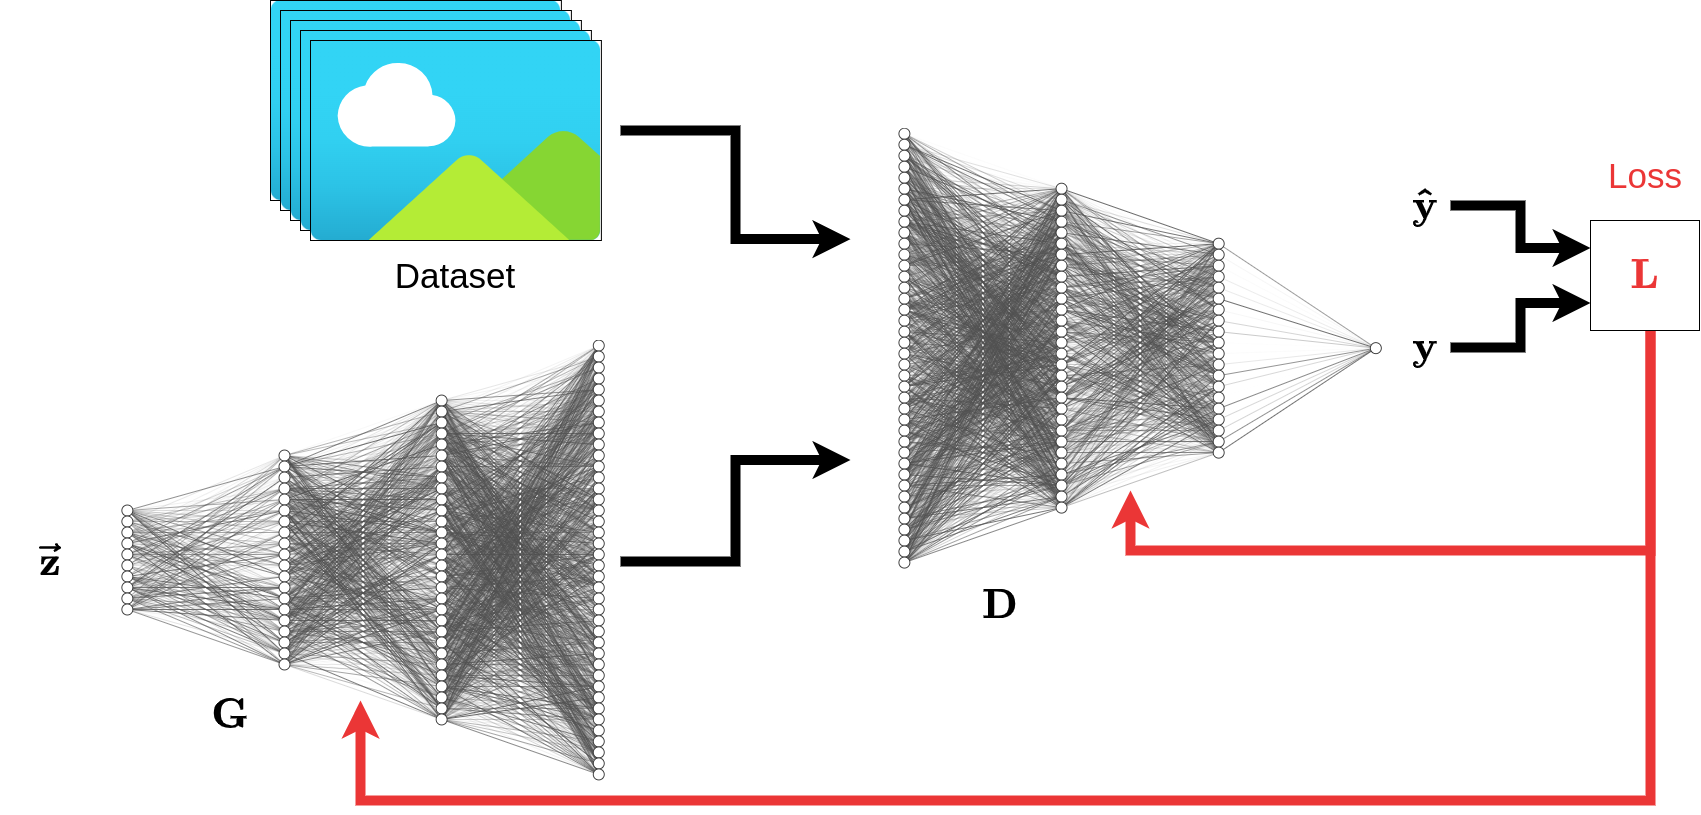
\includegraphics[width=1.0\textwidth]{imgs/GAN_training.png}
        \caption{Rappresentazione grafica della training pipeline di un modello GAN.}
        \label{fig:gan_training}
    \end{figure}

\subsection{La loss function}
L'\textit{adversarial training} si basa su un concetto innovativo, invece di cercare di definire matematicamente una \textit{loss function} in grado
di guidare il generatore durante l'addestramento, cerca di apprenderne una, nello specifico il discriminatore rappresenta la \textit{loss function} che viene addestrata.
Per dare un'idea di che tipo di miglioramento ha introdotto questo approccio facciamo un esempio utilizzando una \textit{loss function} molto utilizzata 
per addestrare modelli generativi prima dell'introduzione dei modelli GAN, la \textit{Mean Squared Error} (MSE).
Questa \textit{loss function}, specialmente per generatori di immagini, portava a dei risultati sfocati e poco realistici, in quanto la MSE non è in grado di catturare
la struttura dei dati, ma solo di portare il generatore verso un punto medio tra i dati del training set, che non necessariamente fa parte della distribuzione,
tale problema è mostrato graficamente nella seguente figura (Figura: \ref{fig:mse_vs_adversarial}).\\

    \begin{figure}[H]
        \centering
        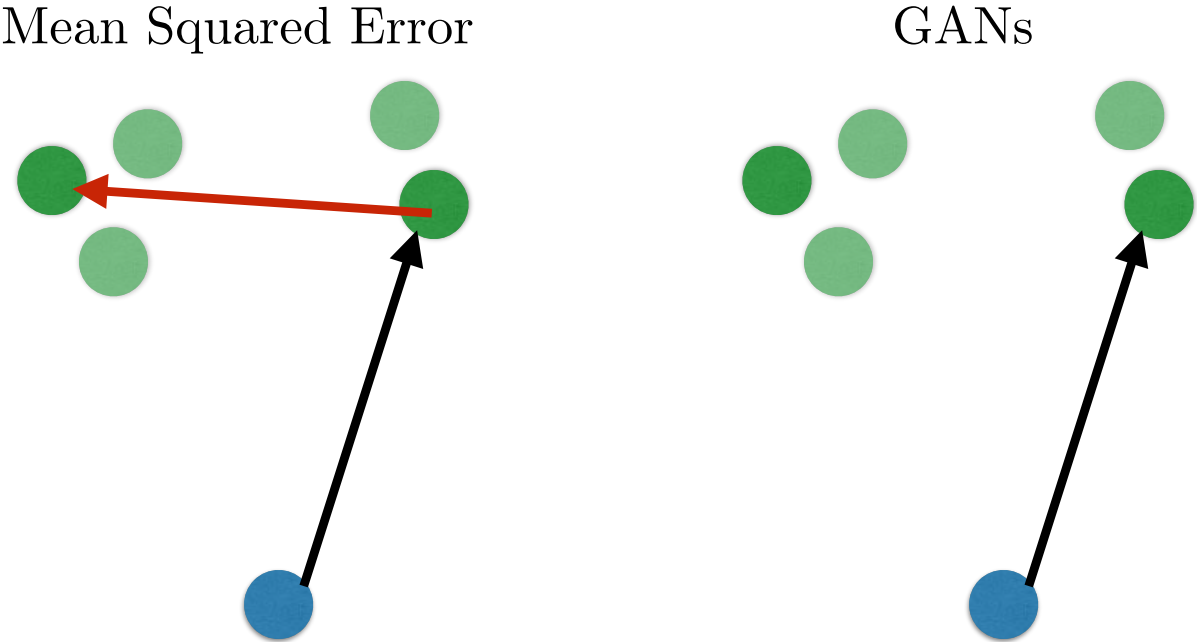
\includegraphics[width=0.5\textwidth]{imgs/mse_vs_adversarial.png}
        \caption{Confronto tra MSE e Adversarial training.\\
        credits: Goodfellow \cite{goodfellow2016ganintro}}
        \label{fig:mse_vs_adversarial}
    \end{figure}

Nella figura possiamo vedere in verde un ipotetico insieme di dati reali e in blu i dati generati dal generatore.
Nel caso del MSE vediamo come il gradiente della loss spinge il generatore verso la zona centrale in quanto punta alla media dei dati reali, 
anche se quella zona non fa parte della distribuzione, mentre nel caso dell'\textit{adversarial training} il gradiente punta verso i dati,
in quanto questa loss è in grado di fare delle considerazioni locali sulla distribuzione dei dati, evitando di cadere in minimi lontani dalla distribuzione reale.\\

Per addestrare il discriminatore e apprendere così una \textit{loss function} aderente ai dati, si è utilizzata come la \textit{Binary Cross Entropy} (BCE), 
utilizzata tipicamente per la classificazione binaria, la quale risulta logicamente adeguata per valutare l'output del discriminatore.\\
La BCE in generale è definita come segue:

\begin{equation}
    \mathbf{BCE(y, \hat{y}) = -\hat{y} \cdot \log(y) - (1-\hat{y}) \cdot \log(1-y)}
\end{equation}

Presenta 2 componenti principali, $\mathbf{-\hat{y} \cdot \log(y)}$ che si attiva quando il risultato atteso è $\mathbf{y = 1}$, mentre l'altra componente si azzera,
e $\mathbf{(1-\hat{y}) \cdot \log(1-y)}$ che si attiva quando il risultato atteso è $\mathbf{y = 0}$, con l'altra componente a 0.

\begin{figure}[H]
    \begin{tabular}{cc}
        % first row
        \vspace{0.15cm}
        \subfloat[Binary Cross Entropy ($\hat{y} = 0$)]{
            \label{fig:BCE_0}
            \centering
            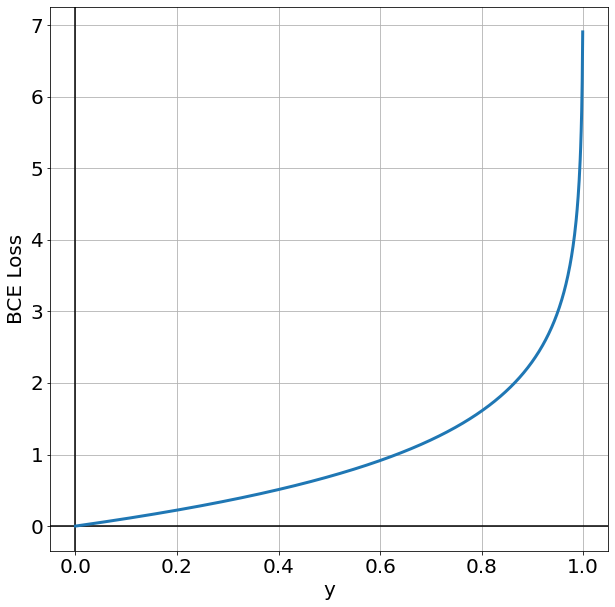
\includegraphics[width=0.425\textwidth]{imgs/graphs/bce_0.png}
        }  &
        \subfloat[Binary Cross Entropy ($\hat{y} = 1$)]{
            \label{fig:BCE_1}
            \centering
            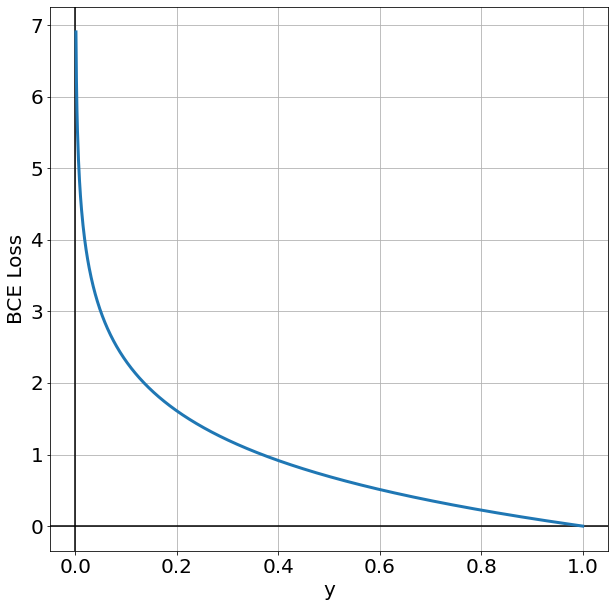
\includegraphics[width=0.425\textwidth]{imgs/graphs/bce_1.png}
        }  \\
        \vspace{0.25cm}
        \subfloat{
            \begin{tabular}{|c|}
                \hline
                $\mathbf{-\log(1-y)}$ \\
                \hline
            \end{tabular}
        } &
        \subfloat{
            \begin{tabular}{|c|}
                \hline
                $\mathbf{-\log(y)}$\\
                \hline
            \end{tabular}
        } \\
    \end{tabular}
\end{figure}

Nel caso dell'addestramento di un modello GAN, possiamo riscrivere la BCE, attuando alcune semplificazioni, e sostituendo $\mathbf{y}$
con il valore corrispondente, nel caso in cui la $\mathbf{y}$ deriva da un sample reale e quando deriva da un sample generato:

\begin{equation}
    \mathbf{\hat{y} = 1 \rightarrow y = D(\theta_D, x)}
\end{equation}

\begin{equation}
    \mathbf{\hat{y} = 0 \rightarrow y = D(\theta_D, G(\theta_G, z))}
\end{equation}

Trasformando la BCE loss in un gioco di minimizzazione e massimizzazione contrapposta tra i due attori, ottenendo la seguente funzione: 

\begin{equation}
    \mathbf{min_G max_D V(D,G) = \mathbb{E}_{x\sim p_{data}}[log(D(x))] + \mathbb{E}_{z\sim p_{z}}[log(1 - D(G(z)))]}
\end{equation}

In generale possiamo riscrivere le due componenti della funzione appena descritta in maniera estesa come segue:

\begin{equation}
    \mathbb{E}_{x\sim p_{data}}[log(D(x))] = \sum_{i=1}^{n} log(D(x_i)), x_i \in \mathbb{D}t
\end{equation}

Dove $\mathbb{D}t = \{x_1, x_2, ..., x_n\}$ è l'insieme degli esempi del training set. Mentre la seconda componente è definita come segue:

\begin{equation}
    \mathbb{E}_{z\sim p_{z}}[log(1 - D(G(z)))] = \sum_{i=1}^{n} log(1 - D(G(z_i))), z_i \sim p_{z}
\end{equation}

L'applicazione di questa funzione però necessita di qualche accorgimento, nella pratica infatti il modello viene addestrato in due fasi distinte e periodiche,
in una viene addestrato il discriminatore, e nell'altra il generatore, per un numero di step predefiniti. 
Tale dinamica di addestramento ha lo scopo di mantenere le uscite
del discriminatore per i dati generati e reali sufficientemente vicine da non causare problemi di saturazione.
Altrimenti la saturazione comporta un azzeramento del gradiente e di conseguenza un arresto dell'apprendimento.

\subsection{La convergenza del generatore}
Per visualizzare meglio le dinamiche dell'addestramento che portano alla convergenza del generatore alla distribuzione del training set 
possiamo utilizzare un grafico, ipotizzando di visualizzare i dati del training set su una sola dimensione,
e di visualizzare sull'asse $y$ la densità di probabilità dei dati e il valore dell'uscita del discriminatore, al variare di $\mathbf{x}$, ossia
della variabile di input del discriminatore, in questo caso unidimensionale ma in generale potrebbe rappresentare immagini, audio video e così via.

\begin{figure}[H]
    \centering
    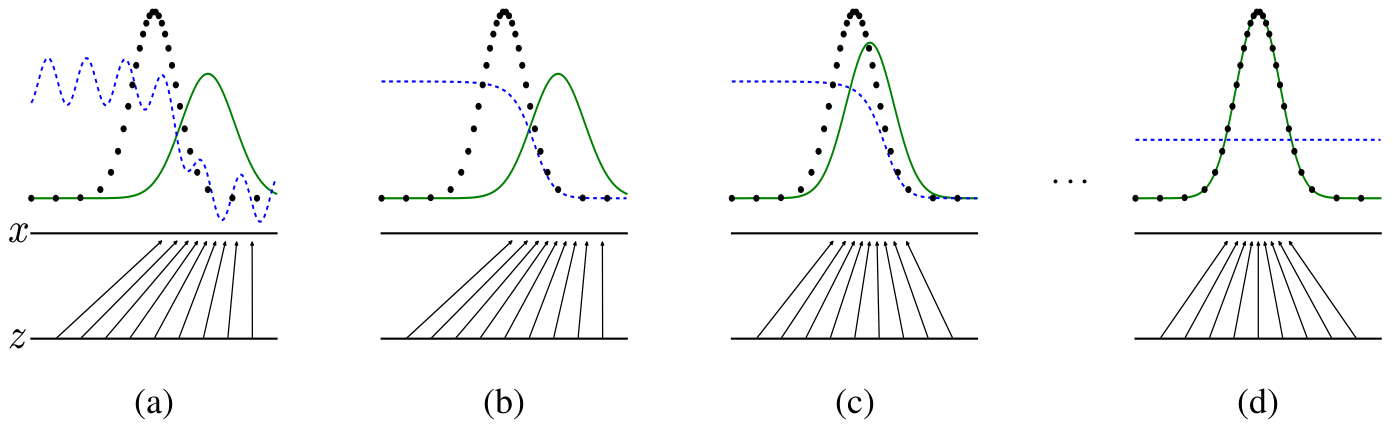
\includegraphics[width=1.0\textwidth]{imgs/Gan training convergence.png}
    \caption{Visualizzazione schematica della convergenza della distribuzione dei dati generati verso quelli reali, e dell'uscita del discriminatore al variare di $\mathbf{x}$.\\
    Si noti che la linea nera tratteggiata rappresenta la distribuzione dei dati reali $p_{data}$, mentre la linea verde continua rappresenta la distribuzione dei dati generati $p_{model}$ e
    in fine la linea blu tratteggiata rappresenta l'uscita del discriminatore $D(x)$, al variare di $\mathbf{x}$. 
    I 2 assi in fondo sono rispettivamente, l'asse $z$ i valori casuali di input del generatore con distribuzione fissa, e l'asse $x$, 
    i valori di input del discriminatore, appartenenti alla distribuzione $\mathbf{p_{data}}$ o $\mathbf{p_{g}}$.\\
    credits: Goodfellow et al. \cite{goodfellow2014generative}}
    \label{fig:gan_training_convergence}
\end{figure}

Nella figura \ref{fig:gan_training_convergence} possiamo vedere diverse fasi dell'addestramento, considerando 4 istanti successivi (a, b, c, d) abbiamo che (a) 
presenta una situazione di apprendimento intermedio in cui il discriminatore comincia ad essere in grado di distinguere con qualche difficoltà i dati reali da quelli
generati e il generatore produce dati piuttosto vicini a quelli reali, in (b) il discriminatore è in grado di distinguere con maggiore precisione i dati reali da quelli
generati, fornendo uno stimolo migliore al generatore, che in (c) è in grado di mappare la distribuzione $\mathbf{p_{z}}$ ad una distribuzione
$\mathbf{p_{g}}$ che tende sempre meglio a quella dei dati reali, infine in (d) possiamo osservare il caso del raggiungimento dell'ottimalità del generatore e dunque la fine dell'addestramento.
In questo caso il discriminatore non è più in grado di distinguere i dati reali da quelli generati, in quanto la distribuzione $\mathbf{p_{g}}$ è sovrapposta 
a quella dei dati reali $\mathbf{p_{data}}$, e si ottiene un'uscita del generatore uguale a 0.5 per ogni valore di input.
La condizione di ottimalità può essere dimostrata, infatti possiamo definire il discriminatore come segue:
\begin{equation}
    \mathbf{D(x) = \frac{p_{data}(x)}{p_{data}(x) + p_{g}(x)}}
\end{equation}

Sapendo che nella condizione ottimale le distribuzioni sono coincidenti $\mathbf{p_{data}(x) = p_{g}(x)}$,
allora considerando $\mathbf{D^*}$ il discriminatore ottimo per un dato $\mathbf{G}$, possiamo scrivere:
\begin{equation}
    \mathbf{D^*(x) = \frac{p_{data}(x)}{p_{data}(x) + p_{g}(x)} = \frac{p_{data}(x)}{2p_{data}(x)} = \frac{1}{2}}
\end{equation}

\subsection{Il gradient vanishing}
\label{subsec:gradient_vanishing}
Il gradient vanishing è un problema che si verifica nel momento in cui il discriminatore riesce a distinguere con troppa facilità i dati reali da quelli generati,
consideriamo infatti che questa è caratterizzata da un singolo elemento dotato di funzione di trasferimento sigmoide, la quale nel
momento in cui restituisce un valore troppo vicino a 0 o 1, ha il gradiente tendente a zero, e di conseguenza dal momento che l'addestramento 
viene effettuato tramite backpropagation, per quanto visto nel capito precedente anche i gradienti dei layer precedenti tenderanno a zero, e l'addestramento
si arresterà. Vediamo di eseguito la funzione di trasferimento sigmoide e il suo gradiente nel momento in cui tende a saturare:

\begin{figure}[H]
    \centering
    \begin{tabular}{cc}
        % first row
        \subfloat[Saturazione per $\mathbf{y \rightarrow 0}$]{
            \label{fig:sig_grad_0}
            \centering
            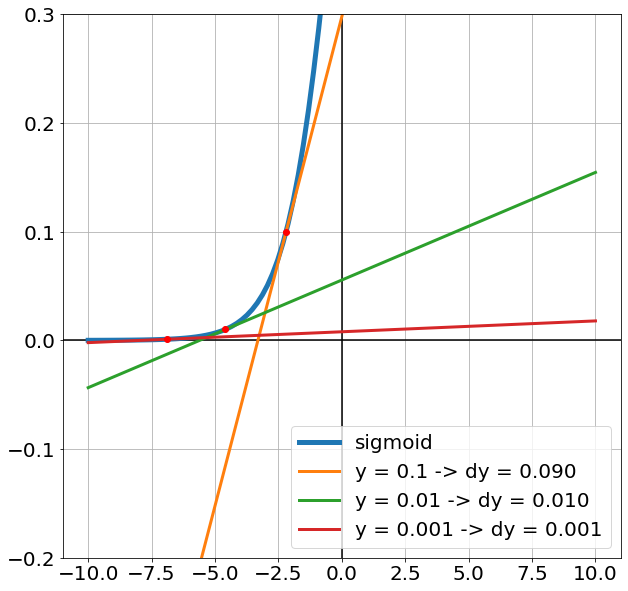
\includegraphics[width=0.4\textwidth]{imgs/graphs/sigmoid_grad_vanish_0.png}
        }  &
        \subfloat[Saturazione per $\mathbf{y \rightarrow 1}$]{
            \label{fig:sig_grad_1}
            \centering
            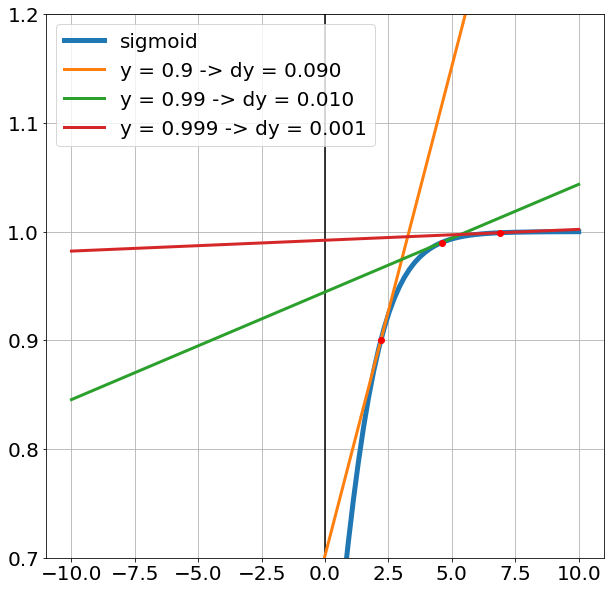
\includegraphics[width=0.4\textwidth]{imgs/graphs/sigmoid_grad_vanish_1.png}
        }  \\
    \end{tabular}
\end{figure}

\subsection{Il mode collapse}
Un'altro problema che affligge i modelli gan è quello del mode collapse, che si verifica quando $\mathbf{G}$ apprende una distribuzione 
che concide con un sottoinsieme di $\mathbf{p_{data}}$. Tale condizione consente comunque di raggiungere
la condizione di ottimalità sopra descritta con $p_{g} \subset p_{data}$, ottenendo comunque $\mathbf{D^*(x) = \frac{1}{2}}$.
Per fare un esempio pratico possiamo considerare ad esempio il dataset Minst che contiene immagini di cifre scritte a mano,
se il generatore impara a generare soltanto cifre dallo 0 al 5 e non quelle dal 6 al 9, siamo in una condizione di mode collapse, 
in quanto parte della distribuzione dei dati non è stata appresa, ma il sistema può comunque raggiungere la condizione di ottimalità.
Nella seguente immagine si ha nella prima riga un esempio di corretto apprendimento mentre nella seconda riga si ha un esempio di mode collapse.
\begin{figure}[H]
    \centering
    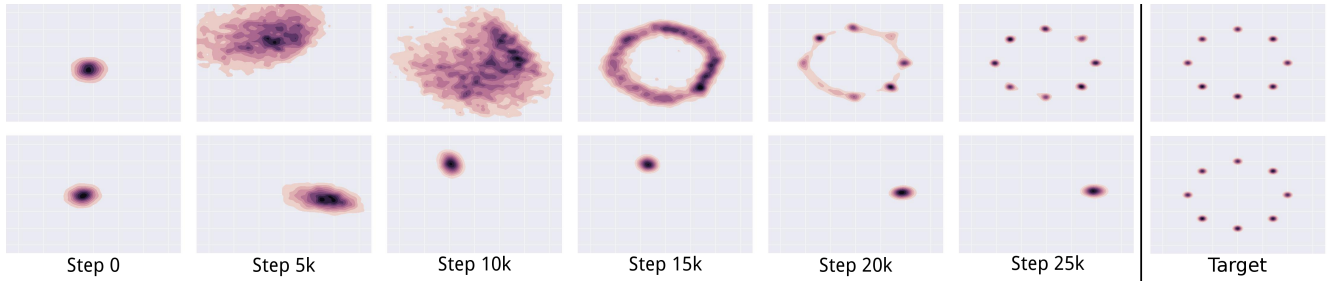
\includegraphics[width=1.0\textwidth]{imgs/mode_collapse.png}
    \caption{Esempio di corretto apprendimento (prima riga) e di mode collapse (seconda riga).\\
    credits: Luke Metz et al. \cite{metz2017unrolled}}
    \label{fig:mode_collapse}
\end{figure}

\subsection{Alcuni risultati}
Vediamo in questa sezione alcuni risultati relativi al modello gan presentato da Goodfellow, relativi a modelli addestrati con
dataset di facce umane in bassa risoluzione e il dataset Minst. In Questi esempi è possibile vedere sulla destra con contorno giallo
alcuni esempi di dati provenienti dal dataset di addestramento, mentre sulla sinistra ci sono gli esempi generati dal modello.

\begin{figure}[H]
    \centering
    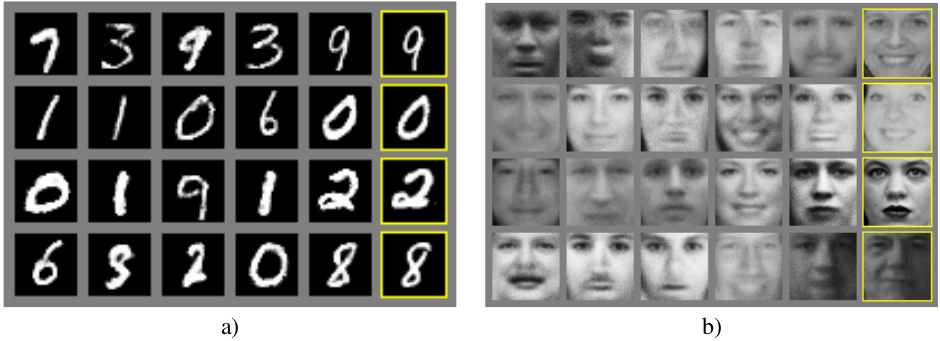
\includegraphics[width=1.0\textwidth]{imgs/first_gan_results.png}
    \caption{Alcuni risultati del modello addestrato in questa ricerca, relativi a un dataset di facce umane in bassa risoluzione (b) e il dataset Minst (a).\\ 
    credits: Goodfellow et al. \cite{goodfellow2014generative}}
    \label{fig:first_gan_results}
\end{figure}

\newpage


%###############################################################################################################################
%###############################################################################################################################
% DCGAN

\section{DCGAN}
DCGAN è stata la prima pubblicazione, opera di Alec Radford et. al \cite{radford2016unsupervised}, che ha dimostrato l'applicabilità dell'adversarial 
training su modelli convoluzionali, ottenendo buoni risultati, aumentando la dimensione delle immagini rispetto a lavori precedenti e mantenendo una buona
efficienza computazionale. Inoltre in questo articolo sono state mostrate per la prima volta le proprietà aritmetiche vettoriali dello spazio latente 
appreso dal generatore durante l'addestramento.

\subsection{L'architettura del modello}
In realtà questo non è stato il primo tentativo di applicare l'adversarial training su modelli convoluzionali, ma il primo ad avere successo.
Altri ci hanno provato prima ma con scarsi risultati, principalmente a causa dell'instabilità del training, che in questo particolare lavoro è 
stata risolta con l'uso di alcuni interessanti accorgimenti.

Rispetto alle implementazioni classiche di convolutional neural network, una scelta interessante è stata quella di rimuovere completamente 
i layer fully connected, eccetto per l'uscita del discriminatore che è un singolo neurone con funzione di attivazione tanh.
Inoltre sono stati rimossi completamente i layer di pooling, sostituiti da semplici layer di convoluzione con stride 2, in modo da dare al modello
la possibilità di apprendere in autonomia come applicare il downsampling nel discriminatore. Nel generatore invece sono stati usati layer di
convoluzione trasposta con stride 2, per ottenere l'upsampling.
Altre note interessanti riguardano l'uso della funzione di attivazione LeakyReLU per il discriminatore e della ReLU per il generatore, e l'uso
della batch normalization per entrambi i modelli, che ha permesso di ottenere una maggiore stabilità del training.

Di seguito vediamo una delle architetture utilizzate in questo articolo per il generatore:

    \begin{figure}[H]
        \centering
        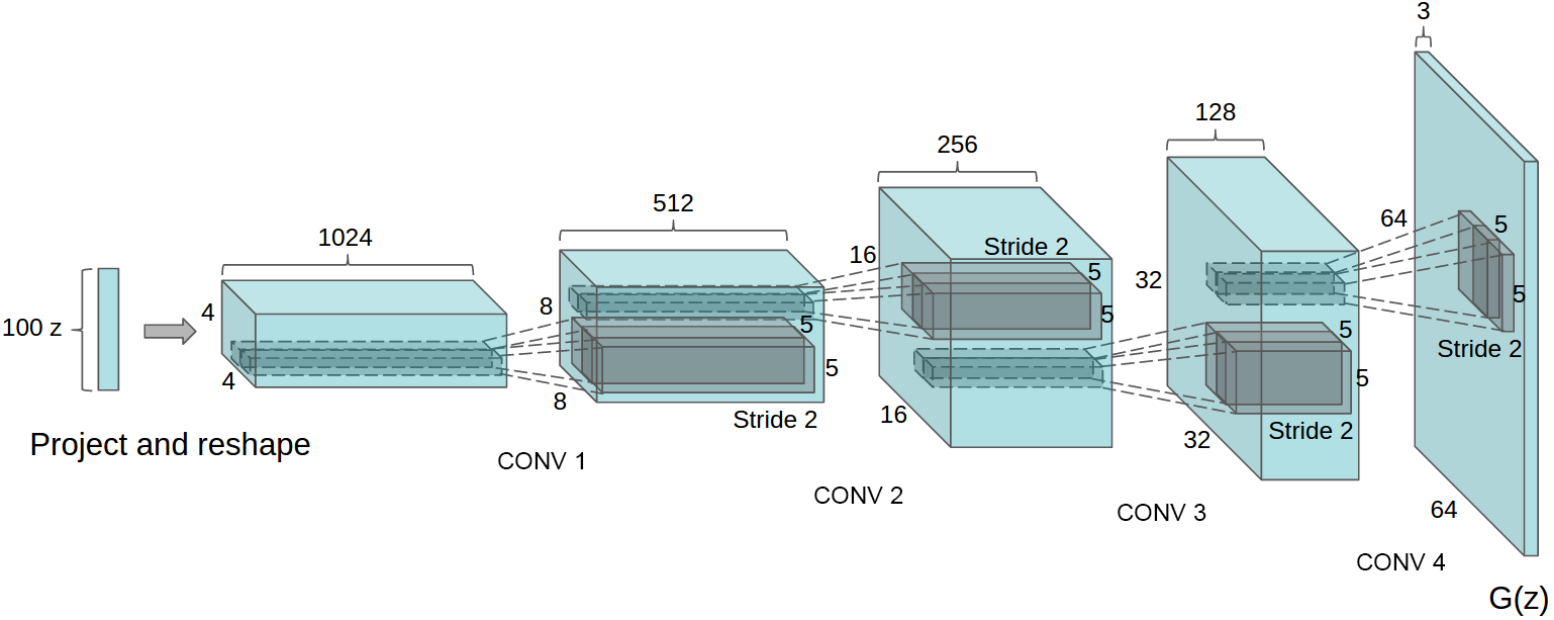
\includegraphics[width=1.0\textwidth]{imgs/DCGAN_generator.png}
        \caption{Architettura del generatore di DCGAN.\\
        credits: Alec Radford et al. \cite{radford2016unsupervised}}
        \label{fig:DCGAN_generator}
    \end{figure}

\subsection{L'algebra vettoriale nello spazio latente Z}
Un'altra proprietà interessante messa in luce da questo articolo sui modelli GAN è il fatto che durante l'addestramento, benché l'input 
$\mathbf{z} \sim \mathbf{p_{z}}$ sia un vettore casuale proveniente da una distribuzione tipicamente gaussiana, il generatore
mostra delle proprietà di auto organizzazione, associando arbitrariamente diverse zone dello spazio latente a diverse caratteristiche 
appartenenti alla distribuzione dei dati reali.
Questo spazio autorganizzato mostra addirittura delle proprietà aritmetiche vettoriali, in quanto sembra possibile effettuare 
operazioni di somma e sottrazione tra i vettori in Z, ed ottenere dei risultati coerenti in termini di immagini. Le stesse semplici operazioni 
effettuate a livello di immagine non danno risultati paragonabili, per tale ragione questo comportamento è indice del fatto che il modello
apprende una rappresentazione dei dati nello spazio latente in maniera profonda e relativa alle caratteristiche che essi presentano, in 
maniera del tutto non supervisionata.

Vediamo un esempio tratto dallo stesso articolo, creato attraverso un modello addestrato su un dataset di facce umane.
Nell'esempio vengono presi 3 vettori per 3 distinte aree di Z: "donna sorridente", "donna seria", "uomo serio" e viene fatta la media 
di questi vettori, ottenendo ancora un vettore che possiede le stesse caratteristiche, ciò indica che queste tre aree sembrano avere una sorta di 
convessità, i vettori mediati vengono poi utilizzati per estrarre la caratteristica "sorridente" e aggiungerla al vettore appartenente all'area "uomo serio",
ottenendo un nuovo vettore che rappresenta un uomo sorridente.
Ciò significa che nello spazio Z è possibile isolare delle caratteristiche e combinarle tra loro per ottenere nuove immagini, lo svantaggio purtroppo
è che lo spazio Z è caratterizzato da una dimensionalità molto elevata, e inoltre queste zone associate a caratteristiche specifiche presentano una elevata
non linearità, per cui in generale è difficile effettuare operazioni di questo tipo con un buon controllo del risultato.

    \begin{figure}[H]
        \centering
        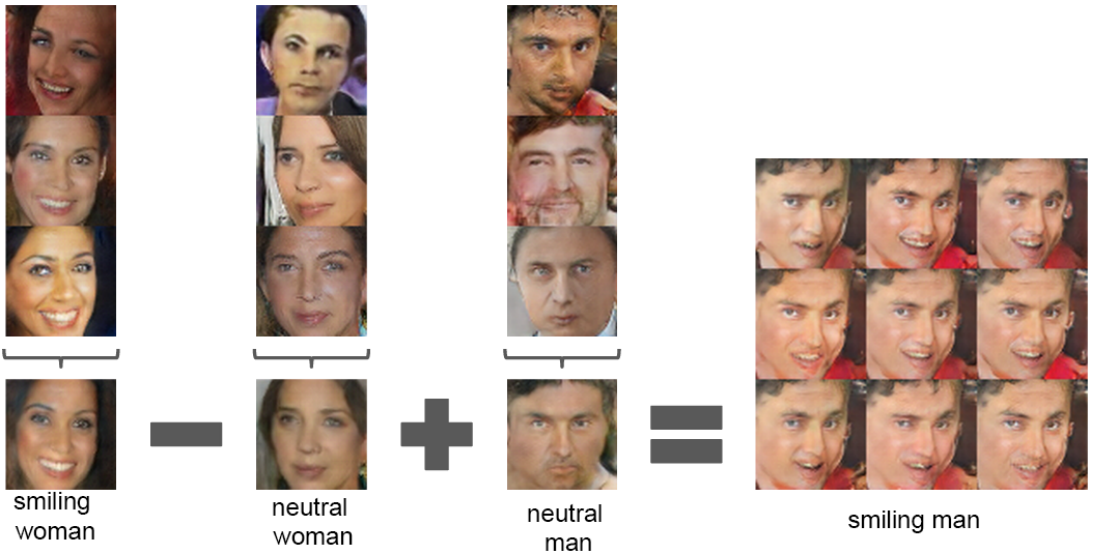
\includegraphics[width=1.0\textwidth]{imgs/DCGAN_vectorial_algebra.png}
        \caption{Esempio di algebra vettoriale nello spazio latente Z.\\
        credits: Alec Radford et al. \cite{radford2016unsupervised}}
        \label{fig:DCGAN_vectorial_algebra}
    \end{figure}

\section{Wasserstein GAN}
Uno dei problemi più seri relativi all'addestramento di un modello neurale attraverso l'\textit{adversarial training},
è la dissolvenza del gradiente durante il training, che porta ad un situazione di stallo in cui il generatore non è più in grado di apprendere.
Tale condizione viene raggiunta nel momento in cui il discriminatore diventa troppo efficacie nel distinguere gli esempi appartenenti al dataset reale
da quelli generati dal generatore, in quel caso come già visto precedentemente nella sezione \ref{subsec:gradient_vanishing}, il gradiente dell'errore
si annulla a causa della saturazione della funzione di attivazione dell'uscita del discriminatore.
Vediamo di seguito un esempio che mette in luce questo problema ipotizzando di avere 2 distribuzioni di dati unidimensionali,
una reale $P_{data}$ e una generata dal generatore $P_{G}$, tali distribuzioni sono affiancate dall'uscita del discriminatore $D(x)$ al variare di $x$.

    \begin{figure}[H]
        \centering
        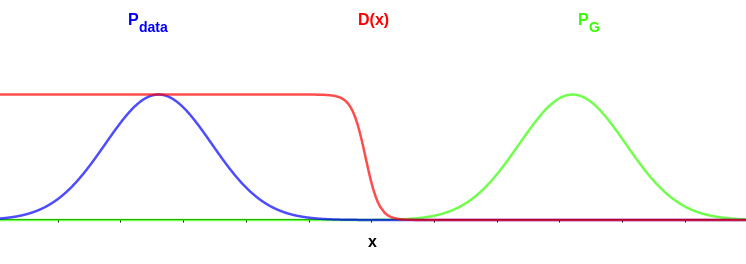
\includegraphics[width=0.7\textwidth]{imgs/wgan_grphs/wgan_graph_1.png}
        \caption{Esempio di \textit{gradient vanishing}, causato da un discriminatore
        addestrato fino all'ottimo per un generatore non ottimo.}
        \label{fig:WGAN_gradient_vanishing}
    \end{figure}

Una soluzione a questo problema è stata proposta da Martin Arjovsky et al. \cite{arjovsky2017wasserstein} nel 2017, i quali hanno introdotto una nuova tipologia
di loss function che permette di evitare il problema del \textit{gradient vanishing} e di ottenere una migliore stabilità del training,
questa rivisitazione del modello GAN è stata chiamata \textit{Wasserstein GAN} (WGAN).
Per comprendere l'innovazione introdotta da questo lavoro dobbiamo dare uno sguardo alla funzione divergenza alla base della funzione di loss del precedente
modello GAN, ovvero la \textit{Jensen-Shannon divergence} (JSD), che è definita come segue:

\begin{equation}
    \label{eq:JSD}
    JSD(P_{data},P_{G}) = \frac{1}{2}KL(P_{data}||\frac{P_{data}+P_{G}}{2}) + \frac{1}{2}KL(P_{G}||\frac{P_{data}+P_{G}}{2})
\end{equation}

Questa metrica permette di misurare la distanza tra due distribuzioni di probabilità, e viene utilizzata in quanto presenta due importanti proprietà,
ovvero è simmetrica ( $JSD(P_{data},P_{G}) = JSD(P_{G},P_{data})$ ) ed è sempre definita.
La $JSD$ è stata introdotta per risolvere le problematiche della $KL$ \textit{Kullback-Leibler divergence}, che non è simmetrica, ovvero ($KL(P_{data}||P_{G}) \neq KL(P_{G}||P_{data})$),
e non è sempre definita. In ogni caso quest'ultima è la formulazione matematica alla base della comunemente utilizzata \textit{cross-entropy loss}. 
vediamo di seguito la definizione della $KL$:

\begin{equation}
    KL(P_{data}||P_{G}) = \sum_{x}P_{data}(x)log\frac{P_{data}(x)}{P_{G}(x)}
\end{equation}

Nonostante la $JSD$ abbia dimostrato la sua efficacia con la precedente formulazione del modello GAN, essa risulta poco sensibile alla distanza 
tra due distribuzioni di probabilità, in particolare quando queste sono molto diverse tra loro, come è possibile vedere graficamente in figura \ref{fig:WGAN_gradient_vanishing}.

\subsection{Earth-Mover distance}
Per risolvere questo problema gli autori hanno formulato una metrica alternativa, chiamata \textit{Earth-Mover distance} (EMD),
che concettualmente misura quanto deve essere spostata una distribuzione per farla coincidere con l'altra.
Concettualmente questa metrica è molto più sensibile di tutte le altre divergenze come la $KL$ e la $JSD$ e altre, in quanto tiene conto della distanza
in maniera lineare. Vediamo di seguito la definizione matematica della $EMD$ per la quale utilizzeremo la notazione $W(P_{data},P_{G})$:

\begin{equation}
    W(P_{data},P_{G}) = \inf_{\gamma \in \prod(P_{data},P_{G})}\mathbb{E}_{(x,y)\sim \gamma}[||x-y||]
\end{equation}

Analizzando le componenti di questa formula possiamo notare che il termine $\prod(P_{data},P_{G})$ rappresenta l'insieme di tutte le possibili distribuzioni
di probabilità $\gamma$ che hanno come marginali le distribuzioni $P_{data}$ e $P_{G}$, ovvero $\gamma$ è una distribuzione di probabilità congiunta.
Per tale ragione il fatto che $W(P_{data},P_{G})$ sia definita come l'estremo inferiore di tutte le possibili distribuzioni congiunte $\gamma$ 
che minimizzano la distanza tra le due distribuzioni $P_{data}$ e $P_{G}$, può essere interpretato come
il percorso minimo che deve essere fatto da una distribuzione per trasformarsi nell'altra.

Il problema di questa formulazione è che non è possibile calcolare direttamente la $EMD$, in quanto non è possibile calcolare la distribuzione 
congiunta $\gamma$ che minimizza la distanza, per tale ragione gli autori hanno proposto una formulazione alternativa che permette di calcolare 
la $EMD$ in maniera approssimata, questa formulazione è la seguente:

\begin{equation}
    \label{eq:Wasserstein_approx}
    W(P_{data},P_{G}) = \sup_{||f||_{L} \leq 1}\mathbb{E}_{x\sim P_{data}}[f(x)] - \mathbb{E}_{x\sim P_{G}}[f(x)]
\end{equation}

L'approssimazione proposta consiste nel calcolare la differenza tra il valore atteso di una funzione $f$ calcolata sui dati reali e il valore atteso
della stessa funzione calcolata sui dati generati dal generatore, dove $f$ è una funzione arbitraria che rispetta la \textit{Lipschitz continuity} con $K=1$, ovvero:

\begin{equation}
    ||f||_{L \leq K} \implies \frac{|f(x)-f(y)|}{|x-y|} \leq K, \forall x \neq y
\end{equation}

In altre parole una funzione che rispetta la \textit{K-Lipschitz continuity} è una funzione che non può avere pendenza (o la derivata) maggiore di $K$ o minore di $-K$,
vediamo di seguito nella figura \ref{fig:lipschitz_continuity} e \ref{fig:lipschitz_continuity2} due funzioni, una che rispetta la \textit{1-Lipschitz continuity} e una no:

    \begin{figure}[H]
        \centering
        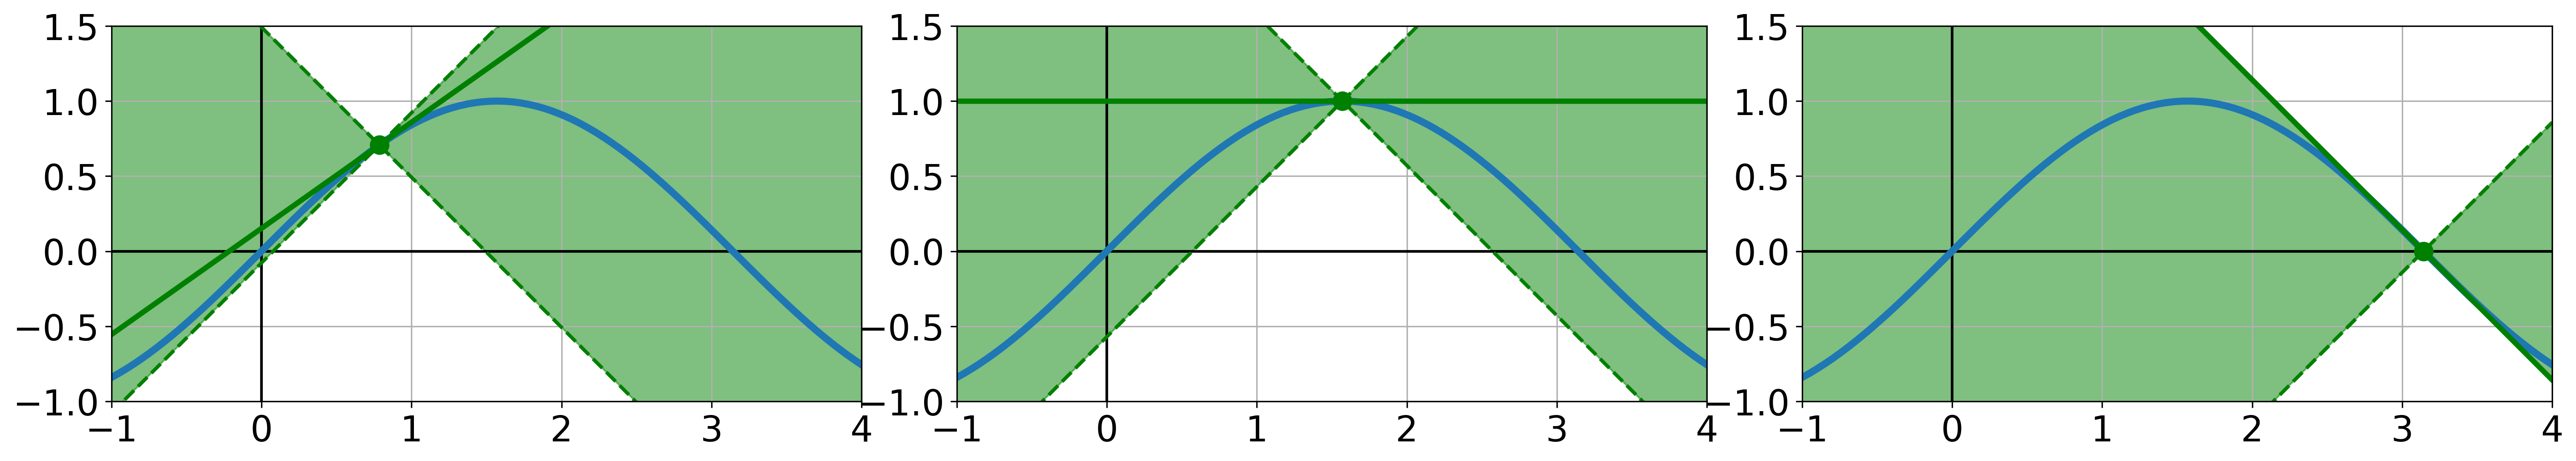
\includegraphics[width=0.8\textwidth]{imgs/graphs/sin_1lipschitz.png}
        \caption{In questa immagine è possibile vedere la derivata della funzione seno, nei punti $\pi/4$, $\pi/2$ e $\pi$,
        ed è possibile vedere come tale funzione rispetta la \textit{1-Lipschitz continuity}, essendo la sua derivata 
        all'interno dell'intervallo ammesso in ogni punto.}
        \label{fig:lipschitz_continuity}
    \end{figure}

    \begin{figure}[H]
        \centering
        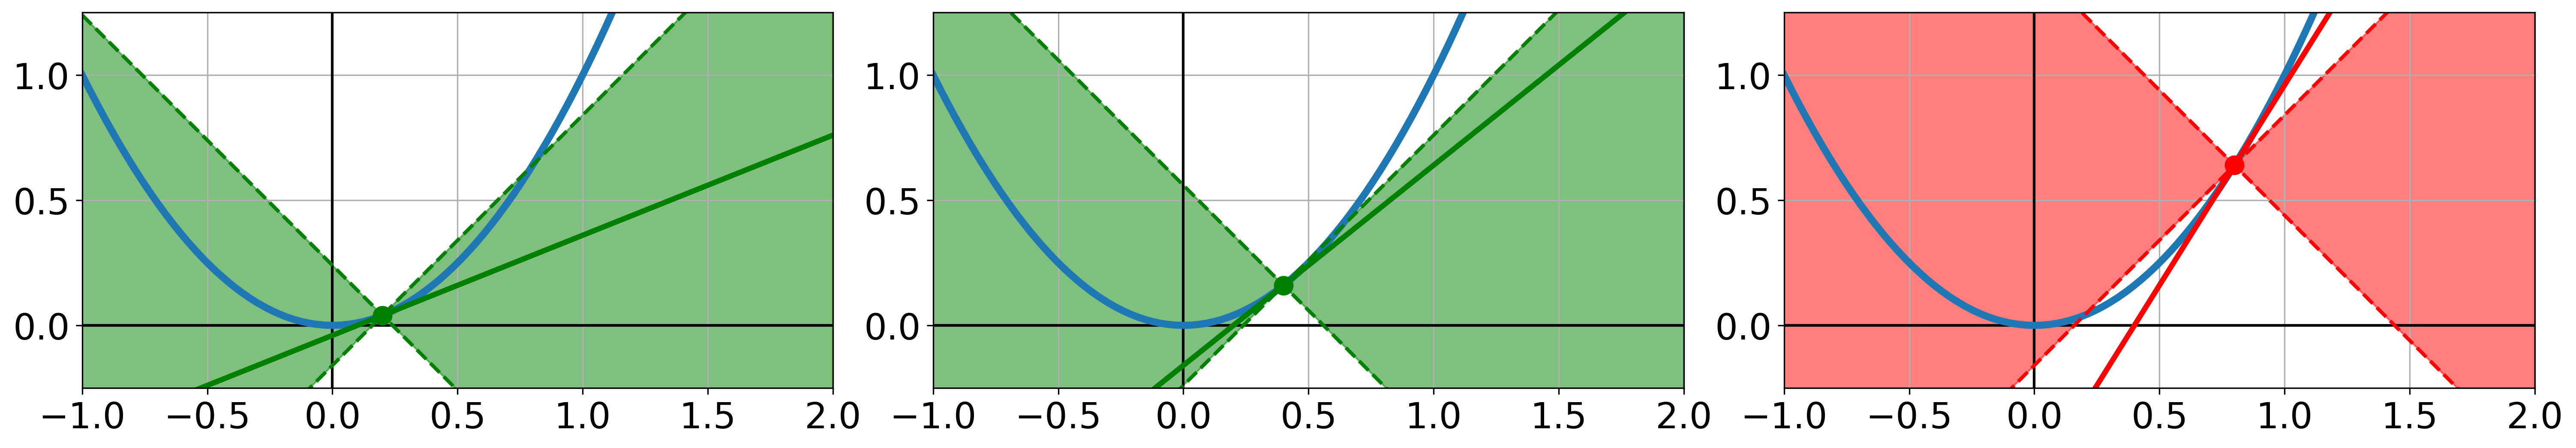
\includegraphics[width=0.8\textwidth]{imgs/graphs/x2_1lipschitz.png}
        \caption{In questa immagine è possibile vedere la derivata della funzione $x^2$, nei punti 0.2, 0.4 e 0.8,
        in questo caso la funzione non rispetta la \textit{1-Lipschitz continuity}, in quanto la sua derivata cresce rapidamente 
        oltre il limite consentito dopo x=0.4.}
        \label{fig:lipschitz_continuity2}
    \end{figure}

La funzione $f$ considerata nella equazione \ref{eq:Wasserstein_approx} è detta \textit{critico}, e prende il posto del discriminatore.
Concettualmente il \textit{critico} e il discriminatore sono uguali eccetto che per l'uscita, infatti il \textit{critico} non ha una funzione di trasferimento
che vincola l'uscita tra 0 e 1, ma può assumere qualsiasi valore reale.
Questa peculiarità gli consente di esprimere la distanza tra due distribuzioni in maniera molto più precisa rispetto al discriminatore,
che a causa dell'equazione \ref{eq:JSD} alla base del suo funzionamento non è in grado di esprimere la distanza tra due distribuzioni in maniera efficacie.
Vediamo di seguito l'immagine \ref{fig:critic} che mostra come il critico sia in grado di mappare molto più efficacemente la distanza tra due distribuzioni,
restituendo dei gradienti utili per il generatore anche quando il critico è addestrato all'ottimo, per il dato generatore.

    \begin{figure}[H]
        \centering
        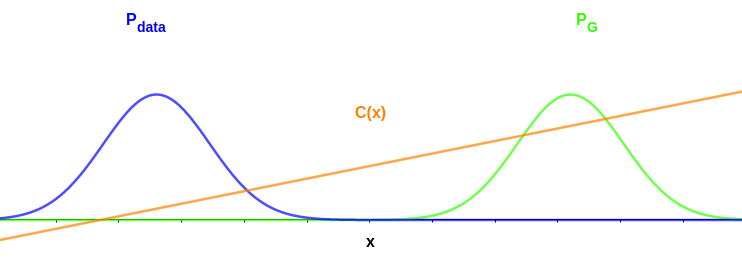
\includegraphics[width=0.8\textwidth]{imgs/wgan_grphs/wgan_graph_2.png}
        \caption{In questa immagine è possibile vedere come il critico $C(x)$ sia in grado di mappare efficacemente la distanza tra due distribuzioni $P_{data}$ e $P_{G}$,
        restituendo dei gradienti utili per il generatore anche quando il critico è addestrato all'ottimo per il dato generatore.}
        \label{fig:critic}
    \end{figure}

Per quanto riguarda la \textit{1-Lipschitz continuity}, fare in modo che un modello neurale la rispetti non è un problema banale, nel quale gli stessi autori
hanno trovato delle difficoltà, proponendo come soluzione il \textit{weight clipping}, ovvero limitare i pesi del critico ad un intervallo di valori,
nello specifico nella paper originale è stato proposto l'intervallo $[-0.01,0.01]$.
Questa soluzione però può portare a problematiche di \textit{vanishing gradient}, un'altra volta, gli autori in ogni caso hanno lasciato aperta
la questione incoraggiando la ricerca di soluzioni alternative, che potessero risolvere il problema in maniera più efficacie e senza effetti collaterali.
Le soluzioni che sono state proposte successivamente per risolvere il problema della \textit{1-Lipschitz continuity} sono state principalmente due:
\begin{itemize}
    \item \textbf{Gradient Penalty}: Questa soluzione consiste nel penalizzare il gradiente del critico
    quando questo assume valori che non rispettano la \textit{1-Lipschitz continuity}.
    \item \textbf{Spectral Normalization}: Questa soluzione consiste nel normalizzare gli autovalori della matrice
    dei pesi del critico.
\end{itemize}

\subsection{Alcuni risultati}
Vediamo di seguito alcuni risultati, che evidenziano l'andamento dell'addestramento di due modelli, una DCGAN e una MLP a 4 strati, con delle immagini
generate durante l'addestramento, e il valore della \textit{loss function}, nell'immagine \ref{fig:wgan_graph_1}so possiamo vedere la 
\textit{Wasserstein distance} e nell'immagine \ref{fig:wgan_graph_2} il caso di addestramento con la \textit{JSD}.
Tale esempio mette in risalto il fatto che la loss proposta dagli autori dimostra una notevole correlazione con la qualità delle immagini generate,
al contrario l'approccio basato su \textit{Jensen-Shannon divergence} non è in grado di fornire un indicatore di qualità delle immagini generate,
in quanto la metrica rimane stabile durante l'addestramento o addirittura cresce mediamente, con il miglioramento della qualità delle immagini generate.

    \begin{figure}[H]
        \centering
        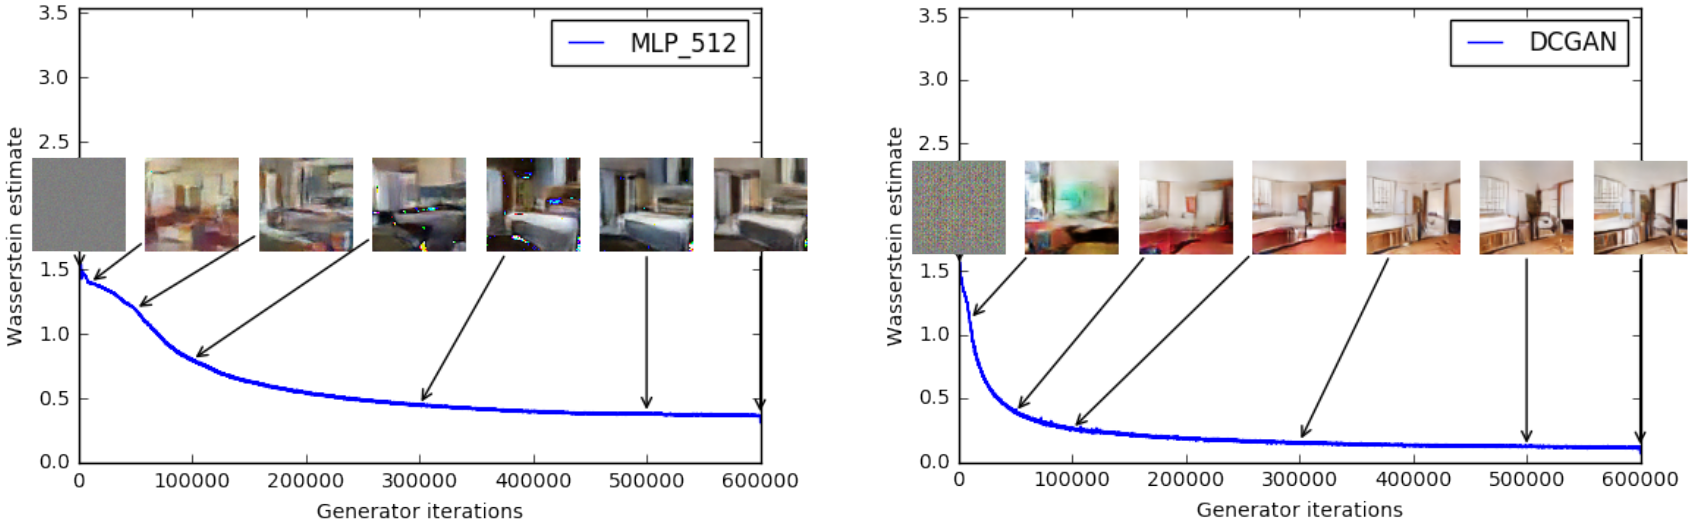
\includegraphics[width=1.0\textwidth]{imgs/wgan_wtrain.png}
        \caption{Andamento del training di una DCGAN e di una MLP addestrate utilizzando la \textit{Wasserstein distance}. 
        credits: Martin Arjovsky et al. \cite{arjovsky2017wasserstein}}
        \label{fig:wgan_graph_1}
    \end{figure}
    \begin{figure}[H]
        \centering
        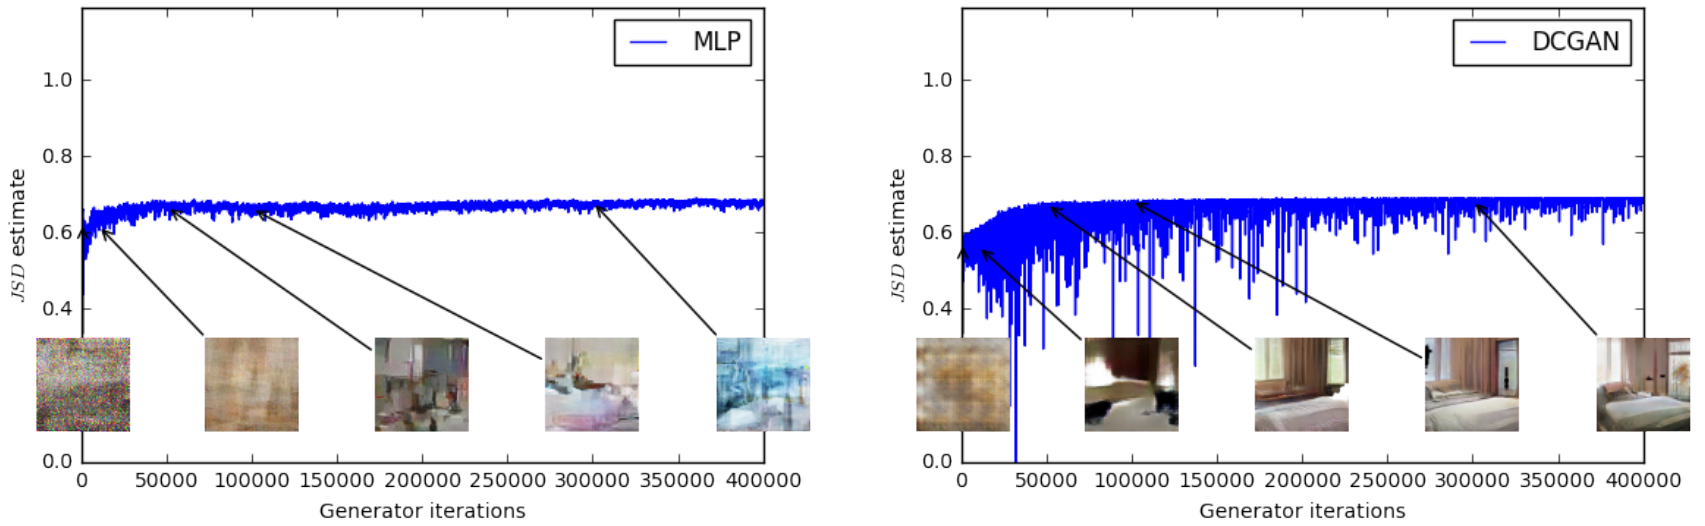
\includegraphics[width=1.0\textwidth]{imgs/wgan_nwtrain.png}
        \caption{Andamento del training di una DCGAN e di una MLP addestrate utilizzando la \textit{Jensen-Shannon divergence}. 
        credits: Martin Arjovsky et al. \cite{arjovsky2017wasserstein}}
        \label{fig:wgan_graph_2}
    \end{figure}

\section{Pix2Pix}
Un'interessante lavoro presentato poco tempo dopo WGAN è stato Pix2Pix da parte di Phillip Isola et al. \cite{isola2018imagetoimage} nel 2018, i quali hanno proposto 
un'interessante architettura per la generazione di immagini a partire da un'immagine di input.
Questa pubblicazione non è stata la prima a presentare un modello che effettuasse la conversione da un'immagine ad un'altra, ma è stata la prima a 
proporne una variante che sfruttasse l'adversarial training e potesse essere applicata a diversi problemi senza necessità di dover riprogettare
l'architettura del modello o la \textit{loss function}.

Molte altre pubblicazioni infatti prima di questa hanno ottenuto risultati molto interessanti per quanto riguarda task che effettuavano la conversione
da un'immagine ad un'altra, come ad esempio: la \textit{colorization}, il \textit{super-resolution}, lo \textit{style transfer}, il \textit{denoising},
il \textit{future frame prediction} e molti altri, tutti però hanno in comune il fatto di essere architetture o framework specializzati, 
realizzati appositamente per quel task, infatti la realizzazione di tali progetti ha richiesto competenze specifiche e un accurato studio del problema.
Pix2Pix invece si propone come un'architettura che può essere applicata a diversi task, senza necessità di dover riprogettare l'architettura del modello
o la \textit{loss function}, ma semplicemente cambiando il dataset di addestramento, in quanto la \textit{loss function} viene appresa in maniera automatica
dal discriminatore durante l'addestramento e la struttura del modello si presta bene a numerosi task.

\subsection{La loss function}
La \textit{loss function} proposta da Pix2Pix è una variante della \textit{loss function} proposta nella pubblicazione originale della GAN \cite{goodfellow2014generative},
infatti nonostante questa paper risulta essere pubblicata quasi un'anno dopo la pubblicazione di WGAN, il metodo non si era ancora imposto come standard per
l'addestramento di modelli GAN.
Sulla base di precedenti lavori infatti in Pix2Pix è stato utilizzato un discriminatore condizionato, ovvero un discriminatore che riceve in input, oltre
all'uscita del generatore o l'immagine proveniente dalla distribuzione obbiettivo, anche l'immagine di input, in modo tale che il discriminatore possa
valutare la qualità dell'immagine generata anche in base a quest'ultima.
Di seguito vediamo l'equazione \ref{eq:pix2pix_loss} che rappresenta la \textit{loss function} proposta per Pix2Pix detta \textit{Conditional Adversarial Loss}:
\begin{equation}
    \label{eq:pix2pix_loss}
    \mathcal{L}_{cGAN}(G,D) = \mathbb{E}_{x \sim P_X,y \sim P_Y}[\log D(x,y)] + \mathbb{E}_{x \sim P_X,z \sim P_Z}[\log(1-D(x,G(x,z)))]
\end{equation}

Si noti che in questa equazione, rispetto al caso classico precedentemente mostrato, spiccano due componenti distinte:
\begin{itemize}
    \item $\mathbf{x}$ è l'immagine di input
    \item $\mathbf{P_X}$ è la distribuzione delle immagini di input
    \item $\mathbf{y}$  è l'immagine di output
    \item $\mathbf{P_Y}$ è la distribuzione delle immagini di output
\end{itemize}

Di seguito è mostrato un esempio di training di Pix2Pix per il task \textit{edges to photo}, il quale propone una rappresentazione grafica
dell'equazione appena mostrata:

    \begin{figure}[H]
        \centering
        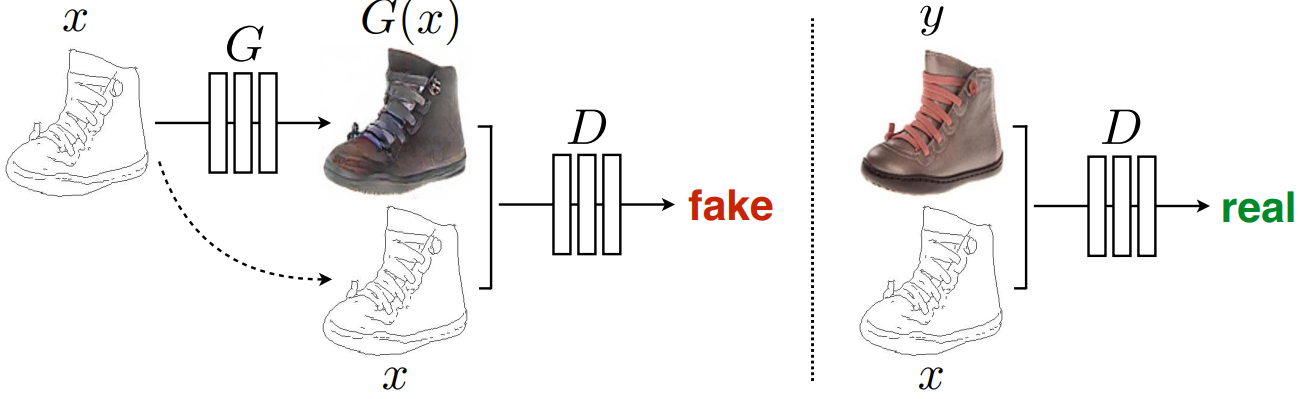
\includegraphics[width=0.8\textwidth]{imgs/pix2pix_train.png}
        \caption{In questa immagine è possibile vedere un esempio di training di Pix2Pix per il task \textit{edges to photo},
        In tale configurazione il discriminatore apprende come discernere tra coppie di immagini e schizzi, e si può vedere come diversamente
        dal caso classico sia il generatore che il discriminatore ricevono in ingresso l'immagine di riferimento (lo schizzo)\\
        credits: Phillip Isola et al. \cite{isola2018imagetoimage}}.
        \label{fig:pix2pix}
    \end{figure}


\subsection{L'architettura}
L'architettura proposta per Pix2Pix utilizza dei blocchi convoluzionali ripresi dalla precedentemente discussa DCGAN \cite{radford2016unsupervised},
composti da tre componenti concatenate \textit{Convolution-BatchNorm-Relu} per ogni layer, sia per il generatore che per il discriminatore.
Per il generatore, nello specifico, è stata ripresa la struttura di U-Net, la quale è stata presentata ed utilizzata con successo per il task di \textit{image segmentation}
da parte di Olaf Ronneberger et al. \cite{ronneberger2015unet} nel 2015.
Tale struttura è in sostanza un \textit{encoder} ed un \textit{decoder} accoppiati con un \textit{bottleneck} centrale, il quale funge 
da ponte tra le due metà e nel quale vengono estratte le informazioni globali dell'immagine, Il decoder in seguito utilizza queste informazioni
per generare l'immagine di output. L'innovazione portata da U-Net è stata quella di aggiungere delle \textit{skip connection} tra l'encoder e il decoder,
in modo da poter utilizzare le informazioni globali estratte al livello del \textit{bottleneck} e di unirle alle informazioni locali presenti nei layer
dell'encoder, in modo tale da poter generare un'output più dettagliato e fedele all'immagine di riferimento. 
Di seguito possiamo vedere la Figura \ref{fig:encoder_decode_unet} che illustra sinteticamente  le differenze tra un modello con struttura ad \textit{encoder-decoder} e U-net.

    \begin{figure}[H]
        \centering
        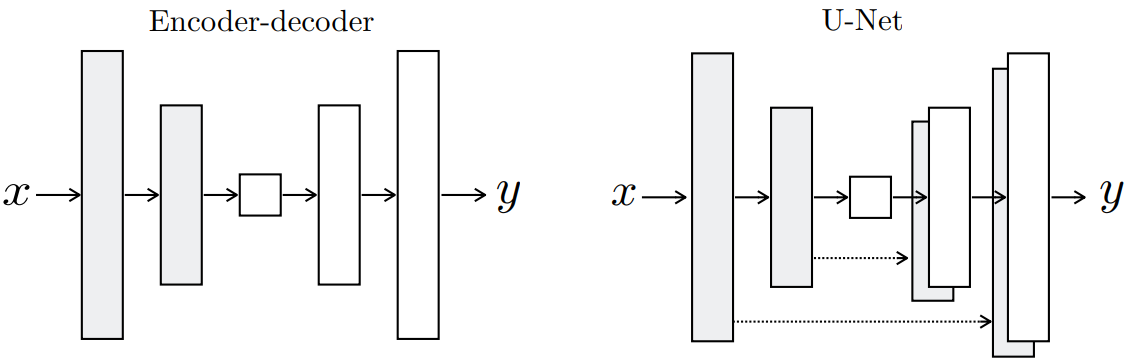
\includegraphics[width=0.7\textwidth]{imgs/encoder_decoder_unet.png}
        \caption{In questa immagine è illustrata intuitivamente la differenza tra un comune modello ad \textit{encoder-decoder} e l'architettura di U-net.\\
        credits: Phillip Isola et al. \cite{isola2018imagetoimage}}.
        \label{fig:encoder_decode_unet}
    \end{figure}

Tale risultato è giustificato dal fatto che, le informazioni dell'immagine di input trovano difficoltà ad essere propagate efficacemente dopo una serie di
\textit{pooling layer}, dunque le \textit{skip connection} permettono di bypassare questi layer e di poter utilizzare le informazioni locali presenti 
nel \textit{encoder}. 
Nella stessa paper sono stati fatti dei test con e senza \textit{skip connection}, e si è visto che l'aggiunta di queste ultime ha portato ad un 
miglioramento delle prestazioni del modello in diversi task. Un chiaro esempio è mostrato in figura \ref{fig:unet_comparison}, 
dove è possibile vedere una comparazione di un sample generato da 4 diversi modelli per il task \textit{labels to scene},
questi quattro modelli alternano l'utilizzo o meno delle \textit{skip connection} e l'utilizzo di una loss L1 a una loss L1 più \textit{conditional adversarial loss}.
    \begin{figure}[H]
        \centering
        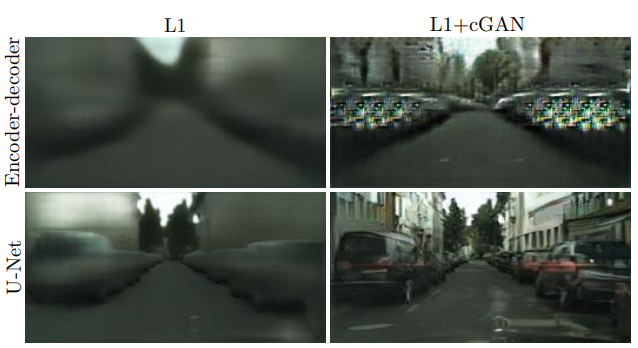
\includegraphics[width=0.8\textwidth]{imgs/unet_comparison.png}
        \caption{In questa immagine è possibile vedere una comparazione di un sample generato da 4 diversi modelli per il task \textit{labels to scene},
            i quattro esempi illustrano l'utilizzo o meno delle \textit{skip connection} e l'utilizzo di una loss L1 a una loss L1 più \textit{conditional adversarial loss}.\\
            credits: Phillip Isola et al. \cite{isola2018imagetoimage}}.
        \label{fig:unet_comparison}
    \end{figure}

\subsection{Alcuni esempi di applicazione}
Di seguito sono mostrati alcuni esempi di applicazione del modello pix2pix, tra i quali: \textit{colorization}, \textit{edges to photo}, \textit{aerial to map},
\textit{labels to scene}, \textit{labels to facade}, \textit{day to night} e \textit{edges to photo}.
    \begin{figure}[H]
        \centering
        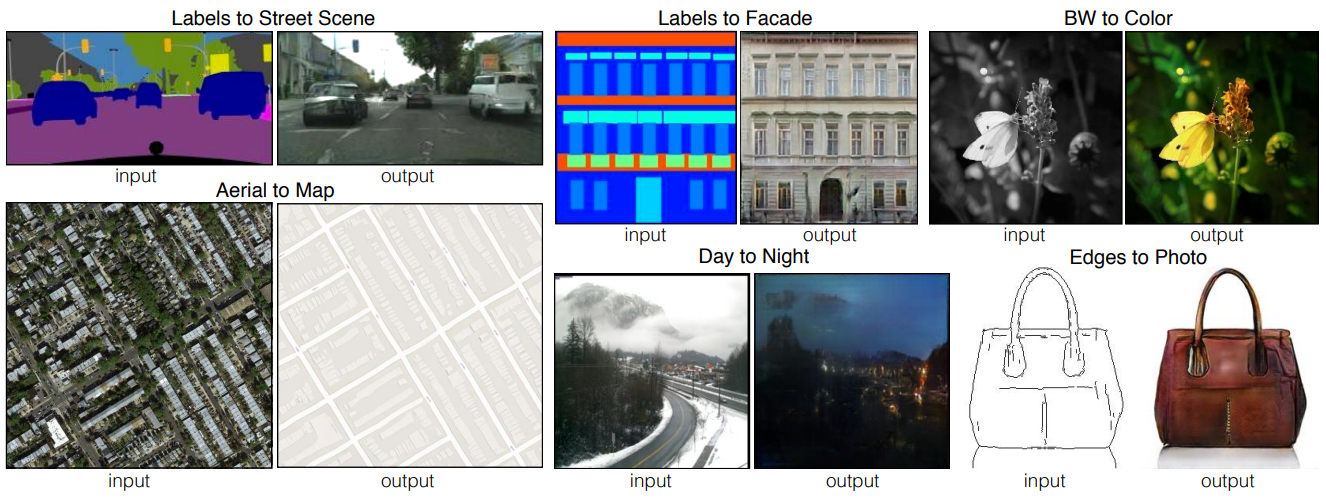
\includegraphics[width=0.85\textwidth]{imgs/pix2pix_example_tasks.png}
        \caption{In questa immagine sono mostrati alcuni esempi di applicazione di pix2pix.\\
            credits: Phillip Isola et al. \cite{isola2018imagetoimage}}.
        \label{fig:pix2pix_example_tasks}
    \end{figure}


\section{LAMA}
\begin{comment}
    Punti chiave di cui discutere per LAMA:
        - Introduzione al task dell'inpainting
        - Struttura del modello e inserto sulla FFC
        - Discussione sulle loss utilizzate
        - Alcuni risultati
        
\end{comment}

Arriviamo in fine al lavoro più recente presentato in questa tesi, e uno dei principali al quale il progetto che verrà illustrato
successivamente è ispirato. LaMa (Large Mask inpainting with fast fourier convolution) è un modello proposto da Roman Suvorov et al. 
\cite{suvorov2021resolutionrobust} nel 2021, tale architettura è stata proposta per il task dell'\textit{inpainting}, il quale consiste
nella ricostruzione di una porzione di immagine mancante, data la restante parte.
LaMa si distingue dagli altri modelli proposti per l'inpainting per una caratteristica peculiare, 
l'utilizzo della \textit{Fast Fourier Convolution} (FFC) \cite{chi2020ffc}, un operatore proposto da Lu Chi et al. nel 2020, la quale
consente di elaborare informazioni globali dell'immagine sin dai primi layer mantenendo
un costo computazionale simile a quello di una convoluzione standard con kernel di dimensioni ridotte. 
Un problema noto delle reti neurali convoluzionali è infatti il legame tra kernel size e receptive field, tanto più sarà grande il kernel size
tanto più velocemente la rete sarà in grado di elaborare informazioni globali, tuttavia ciò comporta un aumento del costo computazionale
che cresce in maniera esponenziale con l'aumentare delle dimensioni del kernel, al contrario la FFC si propone di risolvere questo problema
ad un costo computazionale ridotto, infatti LaMa nei risultati presentati oltre a risultare mediamente migliore rispetto ai concorrenti,
eccelle proprio per i suoi risultati su immagini in cui la parte da ricostruire è molto estesa.

\subsection{Struttura del modello}
In questa sezione vedremo la struttura del modello, analizzando l'input e la struttura dei blocchi principali che lo compongono,
analizzando nello specifico il punto di forza di questa architettura, ovvero l'utilizzo della FFC.

L'input del modello è costituito da un'immagine $x$ e una maschera $m$, dove $m$ è una matrice binaria che ha dimensioni di $x$ ma un solo canale,
e presenta valori 1 nelle posizioni in cui l'immagine è presente e 0 nelle posizioni in cui l'immagine deve essere ricostruita.
Viene quindi effettuata un \textit{element-wise multiplication} tra $x$ e $m$, e si concatena il risultato con $\overline{m}$,
ottenendo il tensore di input $x' = [x \odot m, \overline{m}]$.\\

\begin{figure}[H]
    \centering
    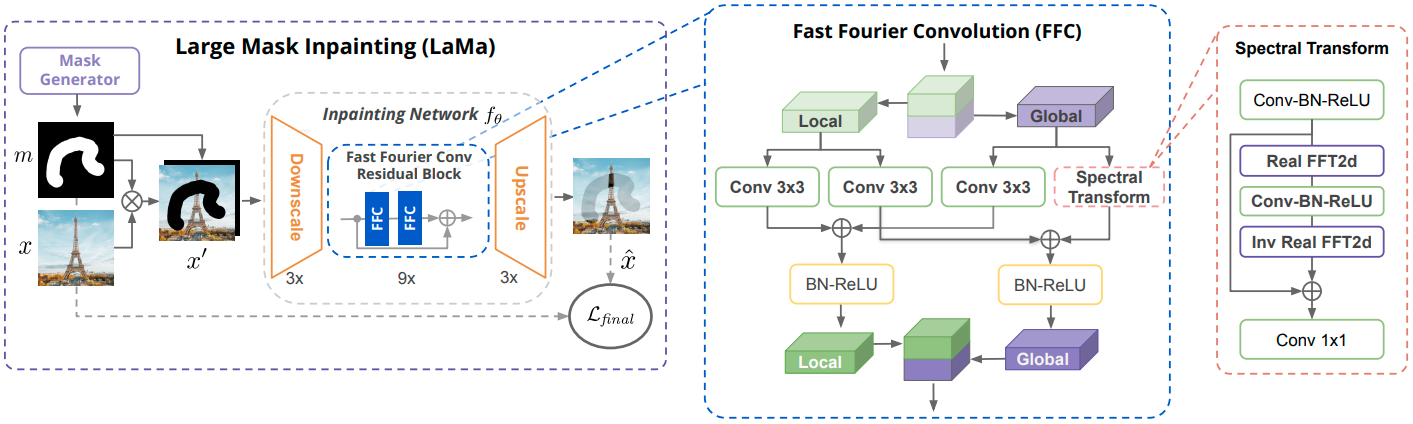
\includegraphics[width=1.0\textwidth]{imgs/lama_model.png}
    \caption{In questa immagine è illustrata schematicamente la struttura di LaMa.\\
        credits: Roman Suvorov et al. \cite{suvorov2021resolutionrobust}}.
    \label{fig:lama_architecture}
\end{figure}

Un'ulteriore operazione che è possibile effettuare per aumentare la variabilità dell'output è quella di aggiungere rumore gaussiano alla matrice
$\overline{m}$, considerando una matrice di rumore gaussiano $z$ con le stesse dimensioni di $\overline{m}$, procedendo come segue:
$ x' = [x \odot m, z \odot \overline{m}]$.



Il modello nella versione base con FCC è costituito inizialmente da 3 blocchi FFC con i seguenti valori stride 2, kernel size 3 e padding 1,
ottenendo dunque per le equazioni [\ref{eq:convolution_output_size_h}, \ref{eq:convolution_output_size_w}] un output di dimensioni dimezzate rispetto all'input
su ogni layer, dunque ottenendo dopo i primi 3 blocchi un output di dimensioni $\frac{1}{8}$ rispetto all'input.\\
Dopo questa prima operazione di downsampling in cui comunque vengono utilizzati blocchi FCC, vengono aggiunti ulteriori 9 blocchi
chiamati dall'autore \textit{Fast Fourier Convolutional Residual Blocks}, costituiti semplicemente da 2 blocchi FCC con stride 1, kernel size 3 e padding 1,
dunque mantenendo le dimensioni dell'input invariato, con in parallelo una connessione residuale che concatena l'input con l'output del secondo blocco FCC,
è possibile osservare il collegamento tra i blocchi FCC nella Figura \ref{fig:lama_architecture}.\\
In fine seguono 3 layer di upsampling, attraverso \textit{transposed convolution} con stride 2, kernel size 3 e padding 1, che riportano l'output alla 
dimensione originale, senza utilizzare blocchi FCC.

\subsubsection{Fast Fourier Convolution}
A questo punto dopo aver snocciolato il contenuto del modello, scendiamo di un'ulteriore livello andando ad analizzare il contenuto dei blocchi FCC,
i quali come visto sopra sono le componenti principali di questa architettura.\\
Prendendo come riferimento il rettangolo tratteggiato in blu in Figura \ref{fig:lama_architecture}, possiamo notare come il tensore in input al
blocco FFC di dimensioni [N, C, H, W] venga diviso in due parti una viene utilizza per l'estrazione delle feature globali e una per l'estrazione delle
feature locali, ovvero un blocco di dimensioni [N, C*(1-$\alpha$), H, W] e un blocco di dimensioni
[N, C*$\alpha$, H, W], dove $\alpha$ è un valore compreso tra 0 e 1, e rappresenta la percentuale di canali che vengono utilizzati per ognuna delle
due componenti.

\begin{table}[H]
    \centering
    \renewcommand{\arraystretch}{1.5} % Imposta il fattore di scala per l'altezza delle righe
    \begin{tabular}{|l|l|l|}
        \hline
        \textbf{Label} & \textbf{Operazione} & \textbf{Dimensioni ingresso uscita} \\ \hline
        \textbf{a} & \textbf{Convolution1x1 $\circ$ BatchNorm $\circ$ ReLU} & $\mathbb{R}^{C \times H \times W} \rightarrow \mathbb{R}^{C \times H \times W}$ \\ \hline
        \textbf{b} & \textbf{Real FFT2d} & $\mathbb{R}^{C \times H \times W} \rightarrow \mathbb{C}^{C \times H \times \frac{W}{2}+1}$ \\ \hline
        \textbf{c} & \textbf{Complex to real} & $\mathbb{C}^{C \times H \times \frac{W}{2}+1} \rightarrow \mathbb{R}^{2C \times H \times \frac{W}{2}+1}$ \\ \hline
        \textbf{d} & \textbf{Convolution1x1 $\circ$ BatchNorm $\circ$ ReLU} & $\mathbb{R}^{2C \times H \times \frac{W}{2}+1} \rightarrow \mathbb{R}^{2C \times H \times \frac{W}{2}+1}$ \\ \hline
        \textbf{e} & \textbf{Real to complex} & $\mathbb{R}^{2C \times H \times \frac{W}{2}+1} \rightarrow \mathbb{C}^{C \times H \times \frac{W}{2}+1}$ \\ \hline
        \textbf{f} & \textbf{Inverse Real FFT2d} & $\mathbb{C}^{C \times H \times \frac{W}{2}+1} \rightarrow \mathbb{R}^{C \times H \times W}$ \\ \hline
        \textbf{g} & \textbf{Concat(a, f)} & $\mathbb{R}^{C \times H \times W} \rightarrow \mathbb{R}^{2C \times H \times W}$ \\ \hline
        \textbf{h} & \textbf{Convolution1x1 $\circ$ BatchNorm $\circ$ ReLU} & $\mathbb{R}^{2C \times H \times W} \rightarrow \mathbb{R}^{2C \times H \times W}$ \\ \hline
    \end{tabular}
    \caption{Operazioni che compongono il sotto blocco \textit{Spectral Transformation}.}
    \label{tab:spectral_transformation}
\end{table}

A questo punto il tensore contenente le informazioni locali (in verde) viene sottoposto a due blocchi convoluzionali standard, mentre il tensore contenente
le informazioni globali (in viola) viene sottoposto ad una operazione di convoluzione standard e ad una operazione detta di \textit{Spectral Transformation},
quest'ultima nello specifico presenta un'operazione in sequenza un operazione di convoluzione standard seguitada un layer per la batch normalization e 
un layer di attivazione ReLU, successivamente viene applicata la \textit{Real Fast Fourier Transform} (RFFT), la quale è una trasformata di Fourier
che opera solo su metà dello spettro. Dopo la trasformazione nel dominio della frequenza, viene applicato un ulteriore layer di convoluzione
(\textit{Convolution-BatchNorm-ReLU}) e successivamente viene applicata la \textit{Inverse Real Fast Fourier Transform} (IRFFT), che è l'inversa della RFFT,
e permette di riportare il tensore a valori reali. Le operazioni del sotto blocco di \textit{Spectral Transformation} sono riassunte nella tabella \ref{tab:spectral_transformation}.

\subsection{La loss function}

L'addestramento di un modello per l'inpainting porta con se una serie di sfide non indifferenti, prima fra tutte è l'ambiguità del task, mentre per altri
la soluzione è unica o comunque limitata ad un numero ristretto di possibilità.
Nel task dell'inpainting i possibili riempimenti per un dato buco in un immagine sono molto numerosi, 
e non è possibile stabilire a priori quale sia la soluzione migliore, specialmente nel caso di aree da rigenerare
di elevata dimensione rispetto all'immagine, ciò rende difficile la definizione di una loss efficacie.

\subsubsection{La perceptual loss PL e la High receptive field perceptual loss HRFPL}
\label{subsubsection:perceptual_loss}

Precedenti tentativi di altri autori di utilizzare loss supervisionate per l'inpainting o la generazione di immagini hanno portato a risultati 
non soddisfacenti, in quanto queste loss tipicamente forzano il generatore a ricostruire l'immagine originale in maniera esatta, 
questo metodo infatti porta il generatore a generare immagini sfocate che sono la media delle possibili soluzioni presentate nel dataset di addestramento.

Un'alternativa alle tradizionali loss supervisionate è data dalla \textit{perceptual loss} proposta per i task di \textit{style transfer}
e \textit{super-resolution} da Justin Johnson et al. \cite{johnson2016perceptual}. Questa particolare loss sfrutta un
modello pre-addestrato $\phi$ per l'estrazione delle feature, in questo modo è possibile definire una loss che misuri la distanza tra le feature
di tale modello, dunque in uno spazio semanticamente più significativo rispetto allo spazio dei pixel, tale proprietà consente alla loss di valutare
la somiglianza semantica tra due immagini, piuttosto che la somiglianza pixel per pixel, permettendo al modello di ricevere un feedback
molto più veritiero sulla bontà del suo output, nonostante questo non sia identico all'immagine originale.\\

Come ben noto all'interno dei modelli convoluzionali si va a creare una stratificazione di feature in cui quelle di basso livello (vicine all'input)
sono associate a caratteristiche locali dell'immagine, mentre quelle di alto livello (vicine all'output) sono associate a caratteristiche globali
come forme o comunque strutture più complesse. Per tale ragione tale loss può essere anche influenzata per dare più peso a caratteristiche globali o locali.

In generale la perceptual loss è definita in \cite{johnson2016perceptual} come:

\begin{equation}
    \mathcal{L}_{\phi}(\hat{y}, y) = \sum_{i=1}^{N} \frac{1}{C_i H_i W_i} \sum_{c=1}^{C_i} \sum_{h=1}^{H_i} \sum_{w=1}^{W_i} \left( \phi_i(\hat{y})_{c,h,w} - \phi_i(y)_{c,h,w} \right)^2
\end{equation}

Tale implementazione della perceptual loss calcola la distanza $L_2$ layer per layer del modello $\phi$ tra l'immagine ricostruita $\hat{y}$ e l'immagine originale $y$ al quadrato,
in tal modo si ottengono $n$ distanze $L_2$ una per ogni layer del modello $\phi$, successivamente si effettua la somma di tali distanze e si ottiene 
la perceptual loss. Una possibile alternativa consiste nell'effettuare la media delle distanze $L_2$ invece della somma, comme mostrato nella
Figura \ref{fig:perceptual_loss} presa da \cite{zhang2018unreasonable}.\\

\begin{figure}[H]
    \centering
    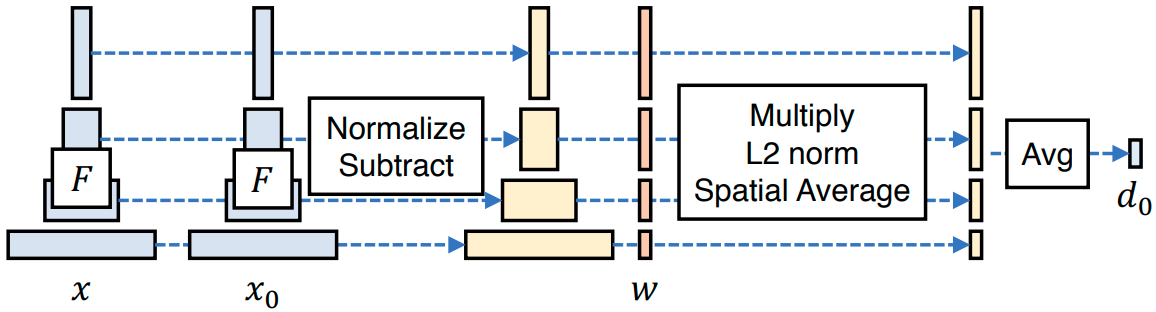
\includegraphics[width=0.9\textwidth]{imgs/perceptual_loss.png}
    \caption{In questa immagine sono mostrati schematicamente i passaggi che permettono di calcolare la perceptual loss da un modello convoluzionale.\\
        credits: Richard Zhang et al. \cite{zhang2018unreasonable}}
    \label{fig:perceptual_loss}
\end{figure}

Per LaMa è stata proposta una variante della PL, denominata \textit{High receptive field perceptual loss} (HRFPL), la quale
presenta le medesime caratteristiche appena descritte per la classica PL ma con la differenza che il modello $\phi$ utilizzato
per il calcolo delle feature presenta delle caratteristiche particolari, ovvero un campo ricettivo esteso come dice il nome stesso (HRF),
tale proprieta può essere ottenuta utilizzando un modello che sfrutti la \textit{dilated convolution} o la \textit{Fast Fourier Convolution} (FFC)
precedentemente illustrata.

\subsubsection{L'adversarial loss}
Un'ulteriore loss utilizzata per l'addestramento di LaMa è la \textit{non-saturating adversarial loss} 

\subsubsection{L'R1 regularization}
TODO

\subsubsection{La loss finale}
TODO

\subsection{Alcuni risultati}
Sono mostrati in seguito alcuni risultati ottenuti da LaMa, in cui è possibile osservare come il modello sia in grado di ricostruire
porzioni di immagine molto estese, e di come l'utilizzo della FFC dia al modello delle eccezionali capacità di ricostruire 
strutture periodiche, come ad esempio le finestre di un edificio, o i fori sulla lamiera di una serranda.
    \begin{figure}[H]
        \centering
        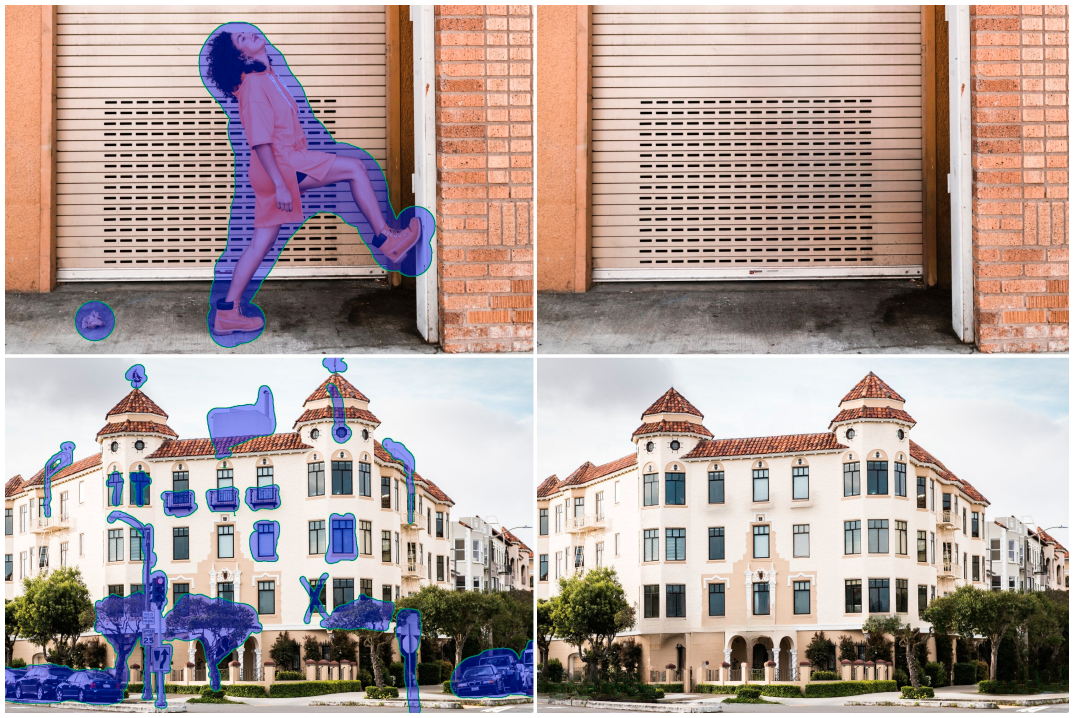
\includegraphics[width=0.9\textwidth]{imgs/lama_results.png}
        \caption{In questa immagine sono mostrati alcuni risultati ottenuti da LaMa. In blu sono 
            rappresentate le maschere applicate alle immagini, e dunque corrispondenti alle arre che sono state rimosse prima
            della propagazione nella rete per la ricostruzione. Le immagini sulla destra rappresentano l'output del modello.\\
            credits: Roman Suvorov et al. \cite{suvorov2021resolutionrobust}}.
        \label{fig:lama_results}
    \end{figure}



